\chapter{Herramienta Web. Back End}
\label{backend}

Fijándonos en el diseño preliminar de la figura \ref{fig:herramienta_web_preliminar} podemos ver que nuestra aplicación Web está dividida en
\emph{front-end} y \emph{back-end}. Esta separación entre módulos es una técnica popular en diseño software. El \emph{front-end} es el encargado de
la capa de presentación, sobre este hablaremos más en el próximo capítulo. En este capítulo nos centraremos en explicar el \emph{back-end}. Este es el
encargado de procesar las peticiones provenientes del \emph{front-end} y devolver le a este la información solicitada. 
\par
El \emph{back-end} será implementado en PHP\cite{PHP}. Este es un lenguaje diseñado para desarrollo Web y además es una elección muy popular. 
Utilizaremos ZendFramework\cite{ZF}, este es un framework orientado al desarrollo de aplicaciones Web. Junto al framework utilizaremos 
Apigility\cite{Apigility}, herramienta que simplifica la creación y mantenimiento de APIs.
\par
Hemos elegido basarnos en la técnica de arquitectura software REST\cite{Rest}, serie de directrices y métodos para crear aplicaciones Web. Los
aspectos básicos de REST a los que más nos ceñiremos son:
\begin{itemize}
	\item	Cliente Servidor. La aplicación debe seguir el modelo Cliente-Servidor. En nuestro caso estas dos identidades son representadas por el
	  	\emph{back-end} y el \emph{front-end}.
	\item	Sin estado. La comunicación entre Cliente y Servidor no mantiene ningún tipo de sesión. La respuesta del Servidor tan solo depende de
	  	la estimulación proporcionada por el Cliente y no es influenciada por los eventos de comunicación anteriores.
	\item	Conjunto bien definido de recursos y operaciones aplicables a esos recursos. En REST por recurso entendemos elementos de información.
	  	Estos recursos serán los solicitados en las peticiones del Cliente. Estos recursos tienen asociada una URL exclusiva que se usa para
		identificarlos.
\end{itemize}
Si nos volvemos a fijar en la figura \ref{fig:herramienta_web_preliminar} podemos ver que en el \emph{back-end} existe la separación entre
\emph{Modelo} y \emph{Controlador}. Esta separación sigue el patrón de diseño MVC\cite{MVCWiki}. Podemos ver que el componente de \emph{Vista} no
existe, en este caso el \emph{front-end} será nuestro componente de \emph{Vista}.
\par
Volviendo a los recursos REST, cada petición recibida por el \emph{back-end} apuntara a un recurso y especificara una operación sobre este. Con el fin
de responder a las peticiones cada recurso tendrá su parte de \emph{Controlador} y \emph{Modelo}. En este capítulo procederemos a explicar los
servicios REST, pero primero explicaremos algunos aspectos técnicos como la base de datos o el ZendFramework.
\section{Protocolo de comunicación}
  	Hemos hablado que entre el \emph{back-end} y \emph{front-end} existe una comunicación. Siendo esta una herramienta Web como es de esperar el
	protocolo de comunicación es HTTP\cite{HTTP}. El \emph{back-end} recibirara \emph{HTTP request} y responderá con \emph{HTTP response}. Las
	peticiones especifican su recurso mediante el URL, al que son anexados los parámetros necesitados. El protocolo ofrece una serie de
	métodos, los más utilizados en este trabajo son \emph{GET} y \emph{POST}. 
	\par
	El método \emph{GET} pide una respuesta del recurso especificado. En función de los parámetros anexados al URL la respuesta cambia.
	\par
	El método \emph{POST} no suele tener parámetros, sin embargo tiene un campo especial. En este cambo se encuentran una serie de datos que serán
	procesados por el \emph{back-end}. Estos datos acabaran creando o actualizando entradas en la base de datos. 
	\par
	Haciendo una pequeña abstracción podemos ver los métodos \emph{GET} y \emph{POST} como \emph{leer y escribir} el recurso especificado.
\section{ZendFramework y Apigility}
	Para la realización de este trabajo utilizaremos ZendFramework, este es un framework orientado al desarrollo de aplicaciones y servicios Web.
	Basado en PHP 5.3+ el framework sigue un diseño orientado a objetos. Esta enfocado para crear aplicaciones siguiendo el patrón MVC. Ofrece
	abstracciones para las bases de datos, autenticación y validación de parámetros. El framework también disfruta de una amplia comunidad de 
	usuarios. Todas estas ventajas nombradas anteriormente son la razón para elegir este framework en nuestro trabajo.
	\par
 	Para  los principiantes el framework ofrece la aplicación esqueleto. Esta aplicación consiste del código mínimo necesario para construir una
	aplicación usando ZendFramework, no tiene ninguna funcionalidad y esta pensada para ser extendida. En este trabajo hemos empezado con esta
	aplicación esqueleto.
  	\par 
  	Apigility es una herramienta creada por el equipo responsable de ZendFramework. La herramienta puede utilizarse sin necesidad del framework,
	sin embargo esta se integra muy bien con este. La herramienta facilita la creación y mantenimiento de aplicaciones Web. En nuestro caso la
	herramienta nos ayudara crear los recursos y métodos de nuestra aplicación REST. La aplicación ofrece un entorno gráfico accesible desde un
	navegador Web. El uso de la herramienta es muy fácil e intuitivo.
\section{Bases de datos}
	Tal y como hemos explicado al principio del capítulo la función del \emph{back-end} es  procesar las peticiones del \emph{front-end} y
	responderle con la información solicitada. Esta información es guardada en dos bases de datos. Para la gestión de las bases de datos
	utilizamos MySql\cite{MySql}. ZendFramework ofrece abstracciones para las bases de datos, esto facilita el trabajo con estas. En la
	figura \ref{fig:tablas} podemos ver el esquema de las tablas con las que vamos a trabajar.
	\par
	En la tabla \texttt{binTable} guardamos la información de las cuentas de cada canal. Junto a esa información guardamos las lecturas del
	barómetro, las fuentes de alta tensión y la fecha y hora actuales. La resolución de los datos es de un minuto.
	\par
	En la tabla \texttt{CALM\_ori} guardamos el valor global y  las correcciones sobre este. La lectura de presión atmosférica también es guardada.
	La resolución de estos datos es también de un minuto.
	\par
	En la tabla \texttt{CALM\_rev} guardamos la revisión de los datos de \texttt{CALM\_ori}. Vemos que la tabla tiene el mismo esquema con dos
	campos adicionales. En estos dos campos se guardan la fecha de última modificación y la versión. Los datos en esta tabla son introducidas por
	un operario. Cuando este encuentra un dato corrupto en los datos originales, puede crear una entrada en esta base de datos para señalarlo.
	\begin{figure}[h]
		\centering
		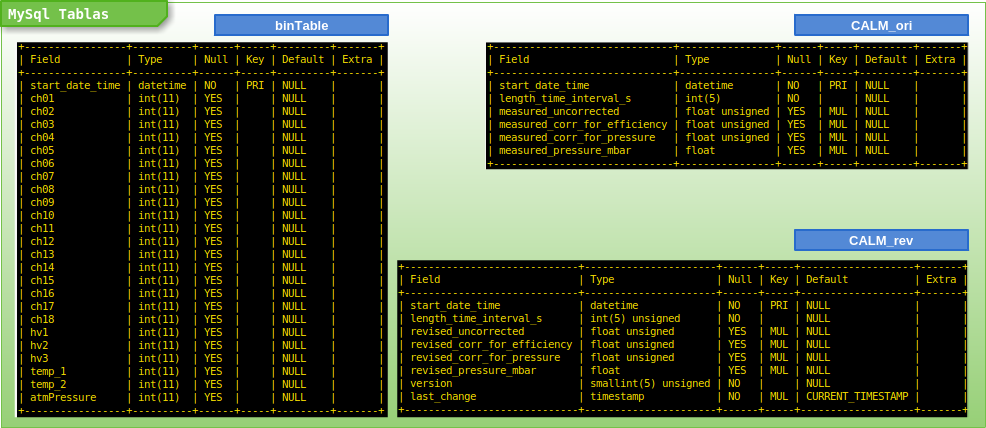
\includegraphics[keepaspectratio, width=1\textwidth]{./img/tablas.png}
		\caption{Esquema de las tablas.}
		\label{fig:tablas}
	\end{figure}
\section{Servicios REST}
  	Es esta sección procederemos a explicar uno a uno los servicios REST que nuestro \emph{back-end} ofrece. Cada servicio REST tiene su parte de
	\emph{Modelo} y \emph{Controlador}. La parte del \emph{Modelo} es la encargada de extraer la información necesaria de la base de datos. El
	\emph{Controlador} es el encargado de procesar las solicitudes, pedirle los datos al controlador y enviar la respuesta al \emph{front-end}.

